\documentclass[11pt,a4paper]{report}

% Packages
\usepackage[utf8]{inputenc}
\usepackage{graphicx}
\usepackage{listings}
\usepackage{color}
\usepackage{hyperref}
\usepackage{amsmath}
\usepackage{tikz}
\usepackage{float}

% Colors for syntax highlighting
\definecolor{codegreen}{rgb}{0,0.6,0}
\definecolor{codegray}{rgb}{0.5,0.5,0.5}
\definecolor{codepurple}{rgb}{0.58,0,0.82}
\definecolor{backcolour}{rgb}{0.95,0.95,0.92}

% Code listing style
\lstdefinestyle{mystyle}{
    backgroundcolor=\color{backcolour},   
    commentstyle=\color{codegreen},
    keywordstyle=\color{magenta},
    numberstyle=\tiny\color{codegray},
    stringstyle=\color{codepurple},
    basicstyle=\ttfamily\footnotesize,
    breakatwhitespace=false,         
    breaklines=true,                 
    captionpos=b,                    
    keepspaces=true,                 
    numbers=left,                    
    numbersep=5pt,                  
    showspaces=false,                
    showstringspaces=false,
    showtabs=false,                  
    tabsize=2
}
\lstset{style=mystyle}

\title{Face Recognition Attendance System\\Technical Documentation}
\author{Technical Team}
\date{\today}

\begin{document}

\maketitle
\tableofcontents

\chapter{System Architecture}

\section{Overview}
The Face Recognition Attendance System is a sophisticated application that combines computer vision, parallel processing, and database management to provide efficient attendance tracking through facial recognition.

\section{Core Technologies}
\begin{itemize}
    \item \textbf{Programming Language:} Python 3.7+
    \item \textbf{GUI Framework:} Tkinter
    \item \textbf{Computer Vision:} OpenCV, InsightFace
    \item \textbf{Database:} SQLite with SQLAlchemy ORM
\end{itemize}

\section{System Components}
\begin{figure}[H]
\centering
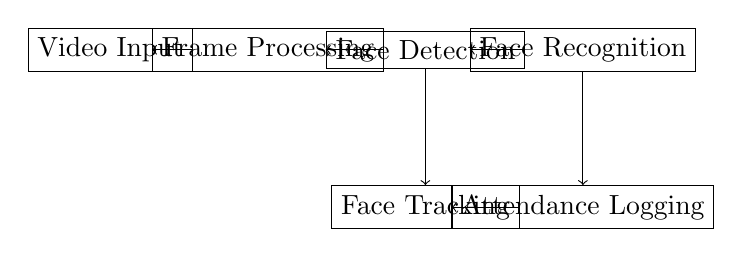
\begin{tikzpicture}[node distance=2cm]
    \node (video) [draw, rectangle] {Video Input};
    \node (process) [draw, rectangle, right of=video] {Frame Processing};
    \node (detect) [draw, rectangle, right of=process] {Face Detection};
    \node (recog) [draw, rectangle, right of=detect] {Face Recognition};
    \node (track) [draw, rectangle, below of=detect] {Face Tracking};
    \node (log) [draw, rectangle, below of=recog] {Attendance Logging};
    
    \draw[->] (video) -- (process);
    \draw[->] (process) -- (detect);
    \draw[->] (detect) -- (recog);
    \draw[->] (detect) -- (track);
    \draw[->] (recog) -- (log);
    \draw[->] (track) -- (log);
\end{tikzpicture}
\caption{System Architecture Overview}
\end{figure}

\chapter{Parallel Processing Architecture}

\section{Thread Pools}

\subsection{Face Detection Pool}
\begin{lstlisting}[language=Python]
class FaceDetectionPool:
    def __init__(self, num_workers: int = 6):
        self.num_workers = num_workers
        self.input_queue = Queue(maxsize=30)
        self.result_queue = Queue()
        self.workers = []
        self.active = True
        self.batch_size = 2
\end{lstlisting}

\subsection{Recognition Pool}
\begin{lstlisting}[language=Python]
class RecognitionPool:
    def __init__(self, num_workers: int = 4):
        self.num_workers = num_workers
        self.input_queue = Queue(maxsize=20)
        self.result_queue = Queue()
        self.face_database = FaceDatabase()
\end{lstlisting}

\chapter{Database Architecture}

\section{Schema Design}
\begin{lstlisting}[language=SQL]
CREATE TABLE users (
    id INTEGER PRIMARY KEY,
    name TEXT NOT NULL,
    created_at DATETIME DEFAULT CURRENT_TIMESTAMP
);

CREATE TABLE face_samples (
    id INTEGER PRIMARY KEY,
    user_id INTEGER,
    image_path TEXT NOT NULL,
    FOREIGN KEY (user_id) REFERENCES users(id)
);

CREATE TABLE attendance (
    id INTEGER PRIMARY KEY,
    user_id INTEGER,
    date DATE DEFAULT CURRENT_DATE,
    check_in_time DATETIME,
    check_out_time DATETIME,
    FOREIGN KEY (user_id) REFERENCES users(id)
);
\end{lstlisting}

\section{Optimization Strategies}
\begin{itemize}
    \item Index Creation
    \item Connection Pooling
    \item Query Optimization
    \item Regular Maintenance
\end{itemize}

\chapter{Face Tracking System}

\section{Motion Predictor}
\begin{lstlisting}[language=Python]
class MotionPredictor:
    def __init__(self):
        self.kalman = cv2.KalmanFilter(4, 2)
        self.initialize_kalman()
        self.last_position = None
        self.confidence = 1.0
        
    def initialize_kalman(self):
        self.kalman.measurementMatrix = np.array([
            [1, 0, 0, 0],
            [0, 1, 0, 0]], np.float32)
\end{lstlisting}

\section{Multi-Scale Tracking}
\begin{lstlisting}[language=Python]
class MultiScaleTracker:
    def __init__(self):
        self.scales = [0.5, 1.0, 2.0]
        self.current_scale = 1.0
        
    def update(self, frame, bbox):
        best_response = float('-inf')
        best_bbox = None
        
        for scale in self.scales:
            scaled_frame = cv2.resize(
                frame, 
                None, 
                fx=scale, 
                fy=scale
            )
\end{lstlisting}

\chapter{Performance Optimization}

\section{Current Metrics}
\begin{itemize}
    \item FPS Range: 10-20 FPS
    \item Detection Pool: 4 worker threads
    \item Frame Buffer Size: 10 frames
    \item Display: LANCZOS resampling
\end{itemize}

\section{Target Metrics}
\begin{itemize}
    \item Target FPS: 45 FPS average
    \item Processing Optimizations: +15-20 FPS
    \item Memory Management: +5-8 FPS
    \item Display Pipeline: +8-10 FPS
\end{itemize}

\section{Optimization Techniques}
\begin{enumerate}
    \item \textbf{Worker Thread Enhancement}
    \begin{itemize}
        \item Increased worker threads
        \item Batch processing implementation
        \item Frame skipping logic
    \end{itemize}
    
    \item \textbf{Memory Management}
    \begin{itemize}
        \item Enhanced frame buffer
        \item Memory pooling
        \item Smart frame dropping
    \end{itemize}
    
    \item \textbf{Display Pipeline}
    \begin{itemize}
        \item Optimized image processing
        \item Frame caching
        \item Efficient color conversion
    \end{itemize}
\end{enumerate}

\chapter{Error Handling and Recovery}

\section{Critical Error Scenarios}
\begin{itemize}
    \item Database Connection Failures
    \item Camera Access Issues
    \item Face Detection Model Errors
    \item Memory Overflow Situations
\end{itemize}

\section{Recovery Procedures}
\begin{lstlisting}[language=Python]
def handle_thread_error(self, thread_id, error):
    try:
        logger.error(f"Thread {thread_id} error: {error}")
        if self._can_recover(error):
            self._restart_thread(thread_id)
        else:
            self._shutdown_gracefully()
    except Exception as e:
        logger.critical(f"Recovery failed: {e}")
        raise
\end{lstlisting}

\chapter{Maintenance Procedures}

\section{Regular Maintenance}
\begin{enumerate}
    \item Database Optimization
    \begin{itemize}
        \item VACUUM operations
        \item Index rebuilding
        \item Statistics update
    \end{itemize}
    
    \item System Monitoring
    \begin{itemize}
        \item Performance metrics collection
        \item Resource usage tracking
        \item Error log analysis
    \end{itemize}
    
    \item Data Management
    \begin{itemize}
        \item Backup procedures
        \item Data cleanup
        \item Storage optimization
    \end{itemize}
\end{enumerate}

\section{Backup Strategy}
\begin{lstlisting}[language=Python]
def backup_database(self):
    timestamp = datetime.now().strftime('%Y%m%d_%H%M%S')
    backup_path = f'backups/database_{timestamp}.sqlite'
    
    connection = sqlite3.connect('database.sqlite')
    backup = sqlite3.connect(backup_path)
    connection.backup(backup)
\end{lstlisting}

\chapter{Future Improvements}

\section{Planned Enhancements}
\begin{enumerate}
    \item GPU Acceleration Support
    \item Cloud Backup Integration
    \item Mobile Application Support
    \item Advanced Analytics Features
\end{enumerate}

\section{Scalability Considerations}
\begin{itemize}
    \item Distributed Processing
    \item Cloud Database Integration
    \item Load Balancing Implementation
    \item Horizontal Scaling Options
\end{itemize}

\end{document}